\begin{table*}[!tb]
\caption{Comparison on five planar sequences (top) and two volumes (bottom). Bold/underline mark best/second distinct values among comparable local measurements only; ties share emphasis. Daggered SNS/TW values are published context and excluded from ranking. Curves use fixed default orientations.}
\label{tab:quantitative-final}
\footnotesize
\setlength{\tabcolsep}{1.5pt}
\renewcommand{\arraystretch}{0.85}
\begin{tabular*}{\textwidth}{@{\extracolsep{\fill}}l*{12}{c}lccc@{}}
\toprule
\multirow{2}{*}{Dataset} & \multicolumn{3}{c}{Hilbert} & \multicolumn{3}{c}{Morton} & \multicolumn{3}{c}{TMTM} & \multicolumn{3}{c}{ST-MTM} & \multicolumn{4}{c}{AnchorMTM (ours)} \\
\cmidrule(lr){2-4}\cmidrule(lr){5-7}\cmidrule(lr){8-10}\cmidrule(lr){11-13}\cmidrule(lr){14-17}
 & SNS$\downarrow$ & TW$\uparrow$ & NPE$\downarrow$ & SNS$\downarrow$ & TW$\uparrow$ & NPE$\downarrow$ & SNS$\downarrow$ & TW$\uparrow$ & NPE$\downarrow$ & SNS$\downarrow$ & TW$\uparrow$ & NPE$\downarrow$ & Mode & SNS$\downarrow$ & TW$\uparrow$ & NPE$\downarrow$ \\
\midrule
\multirow{2}{*}{Gaussian} & \multirow{2}{*}{$0.1117$} & \multirow{2}{*}{$0.6719$} & \multirow{2}{*}{$0.7557$} & \multirow{2}{*}{$\underline{0.0393}$} & \multirow{2}{*}{$\underline{0.8333}$} & \multirow{2}{*}{$0.7359$} & \multirow{2}{*}{$0.25^{\dagger}$} & \multirow{2}{*}{$0.77^{\dagger}$} & \multirow{2}{*}{$\underline{0.1118}$} & \multirow{2}{*}{$0.06^{\dagger}$} & \multirow{2}{*}{$1.00^{\dagger}$} & \multirow{2}{*}{$0.1154$} & Exact & $\mathbf{0.0353}$ & $\mathbf{0.9323}$ & $\mathbf{0.0089}$ \\
 &  &  &  &  &  &  &  &  &  &  &  &  & Balanced & $\mathbf{0.0353}$ & $\mathbf{0.9323}$ & $\mathbf{0.0089}$ \\
\multirow{2}{*}{Ring} & \multirow{2}{*}{$\mathbf{0.1252}$} & \multirow{2}{*}{$0.9048$} & \multirow{2}{*}{$0.5941$} & \multirow{2}{*}{$0.1489$} & \multirow{2}{*}{$0.7619$} & \multirow{2}{*}{$0.6033$} & \multirow{2}{*}{$0.28^{\dagger}$} & \multirow{2}{*}{$0.68^{\dagger}$} & \multirow{2}{*}{$0.1756$} & \multirow{2}{*}{$0.21^{\dagger}$} & \multirow{2}{*}{$0.88^{\dagger}$} & \multirow{2}{*}{$0.2463$} & Exact & $0.1485$ & $0.8571$ & $\underline{0.0471}$ \\
 &  &  &  &  &  &  &  &  &  &  &  &  & Balanced & $\underline{0.1334}$ & $0.8571$ & $\mathbf{0.0395}$ \\
\multirow{2}{*}{Wildfires} & \multirow{2}{*}{$0.1883$} & \multirow{2}{*}{$0.8303$} & \multirow{2}{*}{$0.3641$} & \multirow{2}{*}{$0.1304$} & \multirow{2}{*}{$0.8758$} & \multirow{2}{*}{$0.1560$} & \multirow{2}{*}{$0.44^{\dagger}$} & \multirow{2}{*}{$0.88^{\dagger}$} & \multirow{2}{*}{$0.2280$} & \multirow{2}{*}{$0.24^{\dagger}$} & \multirow{2}{*}{$0.91^{\dagger}$} & \multirow{2}{*}{$0.3180$} & Exact & $\mathbf{0.0426}$ & $0.9136$ & $\underline{0.0131}$ \\
 &  &  &  &  &  &  &  &  &  &  &  &  & Balanced & $\underline{0.0447}$ & $0.8989$ & $\mathbf{0.0116}$ \\
\multirow{2}{*}{Storms} & \multirow{2}{*}{$0.1290$} & \multirow{2}{*}{$0.7403$} & \multirow{2}{*}{$0.3705$} & \multirow{2}{*}{$0.1180$} & \multirow{2}{*}{$0.7251$} & \multirow{2}{*}{$0.3468$} & \multirow{2}{*}{$0.34^{\dagger}$} & \multirow{2}{*}{$0.71^{\dagger}$} & \multirow{2}{*}{$0.5753$} & \multirow{2}{*}{$0.21^{\dagger}$} & \multirow{2}{*}{$0.94^{\dagger}$} & \multirow{2}{*}{$0.4579$} & Exact & $\underline{0.0790}$ & $0.8463$ & $\underline{0.0399}$ \\
 &  &  &  &  &  &  &  &  &  &  &  &  & Balanced & $\mathbf{0.0743}$ & $0.8766$ & $\mathbf{0.0140}$ \\
\multirow{2}{*}{PM2.5} & \multirow{2}{*}{$0.2386$} & \multirow{2}{*}{$\mathbf{0.8887}$} & \multirow{2}{*}{$0.8090$} & \multirow{2}{*}{$\underline{0.1760}$} & \multirow{2}{*}{$\underline{0.8277}$} & \multirow{2}{*}{$0.8823$} & \multirow{2}{*}{$0.3018$} & \multirow{2}{*}{$0.7781$} & \multirow{2}{*}{$0.5241$} & \multirow{2}{*}{$0.1897$} & \multirow{2}{*}{$0.8224$} & \multirow{2}{*}{$0.5577$} & Exact & $0.1964$ & $0.7884$ & $\underline{0.1390}$ \\
 &  &  &  &  &  &  &  &  &  &  &  &  & Balanced & $\mathbf{0.1636}$ & $0.7657$ & $\mathbf{0.0468}$ \\
\midrule
\multirow{2}{*}{Cylinder} & \multirow{2}{*}{$0.2798$} & \multirow{2}{*}{$0.7902$} & \multirow{2}{*}{$0.3700$} & \multirow{2}{*}{$0.2071$} & \multirow{2}{*}{$0.8008$} & \multirow{2}{*}{$0.2810$} & \multirow{2}{*}{$0.2956$} & \multirow{2}{*}{$0.8017$} & \multirow{2}{*}{$0.4769$} & \multirow{2}{*}{$0.1346$} & \multirow{2}{*}{$\underline{0.8989}$} & \multirow{2}{*}{$0.5160$} & Exact & $\underline{0.1097}$ & $0.8136$ & $\underline{0.0918}$ \\
 & & & & & & & & & & & & & Balanced & $\mathbf{0.0405}$ & $\mathbf{0.8998}$ & $\mathbf{0.0133}$ \\
\multirow{2}{*}{Tangaroa} & \multirow{2}{*}{$0.3429$} & \multirow{2}{*}{$\mathbf{0.9222}$} & \multirow{2}{*}{$0.2646$} & \multirow{2}{*}{$0.3627$} & \multirow{2}{*}{$\underline{0.8893}$} & \multirow{2}{*}{$0.4486$} & \multirow{2}{*}{$0.5255$} & \multirow{2}{*}{$0.6701$} & \multirow{2}{*}{$0.3866$} & \multirow{2}{*}{$0.1655$} & \multirow{2}{*}{$0.8137$} & \multirow{2}{*}{$0.3286$} & Exact & $\underline{0.1518}$ & $0.8061$ & $\underline{0.0861}$ \\
 & & & & & & & & & & & & & Balanced & $\mathbf{0.1364}$ & $0.8476$ & $\mathbf{0.0465}$ \\
\bottomrule
\end{tabular*}
\vspace{2pt}
\begin{minipage}{\textwidth}\footnotesize For the original four inputs, TMTM/ST-MTM Temporal SNS/TW ($\dagger$) are published values; other entries are local measurements. The four inputs are our reconstructions (Section~\ref{sec:experiments}). TW needs enough features per frame: 64/64, 1/40, 4/32 and 11/744 frames are eligible on Gaussian, Ring, Wildfires and Storms, so TW is not ranked on the last three. Published TW has two-decimal precision. Mode applies only to AnchorMTM. PM2.5 uses 744 shared-input local frames (TW $k=1$, full coverage); its Balanced mode uses the fixed exploratory 5\% case budget, without validation-set budget selection. ST-MTM uses the Storms preset with start frame 0; PM2.5 baseline metrics are all recomputed. Volumes: all entries local, streamwise $x$ reference, TW $k=1$; Balanced is 1\% (Cylinder) and 9\% (Tangaroa) by the planar rule, attaining 0.99\% and 9.0\% merge error. ST-MTM was not proposed for volumes; its volume rows are our adaptation (Section~\ref{sec:experiments}).\end{minipage}

\end{table*}


\section{Evaluation}\label{sec:experiments}
The evaluation follows the argument of the paper. We first test the bounds and use them to measure how much of the error of existing maps the tree actually forces; this evidence does not depend on what AnchorMTM optimizes. We then ask whether the anchored axis reaches its goal and what that costs in relative geometry and temporal behavior, examine how a merge budget changes individual frames, and read an anchored map against its source field.

\subsection{Data and Measures}
\paragraph{Data.} The four planar sequences are Ring (40 frames), Wildfires (32) and Storms (744), our reconstructions of the ST-MTM benchmark~\cite{STMTM:2026} at its per-frame persistence fractions, because its processed arrays are not available, and hourly PM$_{2.5}$ over northern China in January 2017 (744 frames, 5\% persistence)~\cite{Kong:2021:CAQRA}; Storms uses ERA5 sea-level-pressure anomalies~\cite{Hersbach:2020:ERA5} and Wildfires aggregated fire radiative power~\cite{Franke:2021:1DP}. We omit the Gaussian sequence of that benchmark, which has three features per frame and no conflict between hierarchy and position. The volumes are the flow past a square cylinder (102 frames of the $Q$-criterion, 2\% persistence)~\cite{Camarri:2005:Cylinder,Weinkauf:SquareCylinder} and the Tangaroa ship wake (201 speed fields, absolute persistence 0.2)~\cite{Popinet:2004:Tangaroa}. Within each comparison, all methods share the fields, trees, identities and references.

\paragraph{Compared maps.} TMTM and ST-MTM keep the tree but define no origin or direction for their axis, so each is reflected once per sequence to agree with the reference. ST-MTM was proposed for planar data, and its authors make no claim about volumes; because it is the only existing map that optimizes relative geometry and its inputs do not depend on the dimension, we include our own 3-D adaptation, with 3-D distances and the method's general parameters and without tuning (Supplementary Section~S4.2). Its volume rows report this adaptation, not a result of its authors. The Hilbert and Morton space-filling curves are references for neighborhood quality only: they order all samples of the domain and break the tree, and a curve index corresponds to no spatial direction, so we report no NPE for them and do not rank them.

\paragraph{Measures.} Table~\ref{tab:measures} lists the measures. NPE is our own: AnchorMTM optimizes it and TMTM and ST-MTM do not, so it shows whether the anchoring goal is reached and does not rank the maps in general. The bound and the measures from prior work do not depend on it. SNS and TW compare anchor distances with support-centroid distances; for the three benchmark inputs, the published TMTM and ST-MTM values are quoted for context (daggers in Table~\ref{tab:quantitative-final}). TW needs enough features per frame and is not ranked on Ring, Wildfires and Storms, where only 1, 4 and 11 frames are eligible.

\begin{table}[!tb]
\centering
\caption{Measures of the evaluation. Lower is better, except for TW (higher) and TD (no preferred value, since features do move).}
\label{tab:measures}
\footnotesize
\setlength{\tabcolsep}{3pt}
\renewcommand{\arraystretch}{0.95}
\begin{tabular}{@{}lp{.68\columnwidth}l@{}}
\toprule
Measure & Meaning & Source\\
\midrule
$\nu^*$ & Smallest order error the tree forces (Eq.~\ref{eq:nu}) & this paper\\
NROE & Order error: least worst displacement of a leaf order (Eq.~\ref{eq:nroe}) & this paper\\
NPE & Worst displacement of the drawn map (Eq.~\ref{eq:nroe}) & this paper\\
Merge & Largest change of a displayed merge level (Eq.~\ref{eq:dtop}) & \cite{Munch:2019:LINF}\\
SNS & Scale-normalized stress of distances & \cite{Smelser:2025:Scale}\\
TW & Trustworthiness of neighbors & \cite{Venna:2001:NP}\\
TD & Summed displayed motion of matched anchors & \cite{STMTM:2026}\\
ME & Share of feature pairs whose displayed approach or separation contradicts the true one & --\\
\bottomrule
\end{tabular}
\end{table}

\paragraph{Modes.} Exact uses zero allowance. Balanced uses a positive budget selected once from 1--10\% on the first chronological quarter of each benchmark input (1, 5 and 10\%); PM$_{2.5}$ uses a fixed 5\%. The volumes use the default configuration, the same Balanced rule and the streamwise axis of both flows as a supplied direction (Section~\ref{sec:reference-model}; Supplementary Section~S4.7 gives Tangaroa along its motion); Table~S1 lists the other settings.

\begin{figure*}[!tb]
\centering
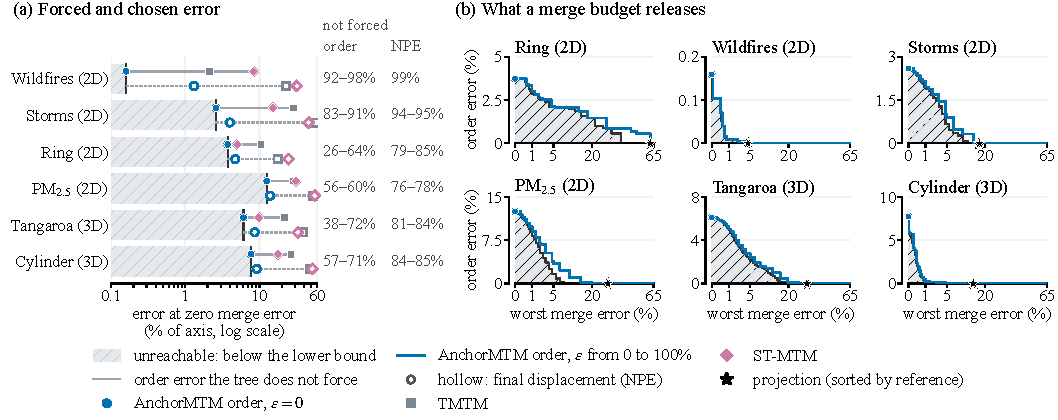
\includegraphics[width=\textwidth]{figures/forced_plane.pdf}
\caption{Forced and chosen error. (a)~The steps of Section~\ref{sec:bounds} for maps that keep the tree (log scale). The hatched region is what the tree forces: no exact map can lie below the bound $\nu^*$. Filled markers are the order error of each map, hollow markers its final displacement NPE. Midpoint ordering (blue, filled) lies on the bound; TMTM and ST-MTM lie far above it. The right columns give the share of TMTM and ST-MTM error above the bound. (b)~The bound as the merge error grows (Proposition~\ref{thm:chain} and the flattened bound), each panel scaled to its own bound. The budgeted point-model order of AnchorMTM ($\varepsilon$ from 0 to 100\%; worst merge error on a square-root scale) runs along it; the projection keeps every reference but breaks the tree.}
\label{fig:plane}
\end{figure*}
\begin{figure*}[!tb]
\paperfigure[\textwidth]{figures/volume_gallery.pdf}{fig:volume-gallery}{Where each map draws the features of Tangaroa and Cylinder along the streamwise axis; the TMTM, ST-MTM and $\varepsilon=0$ columns are the runs of Table~\ref{tab:quantitative-final}. The first column is the reference $q$, the actual location of each feature along $a^*$ and the target of the comparison; light grey dots repeat it in the other panels, and color shows how far a feature is drawn from it. The bars give NPE, the worst displacement of a frame averaged over frames (\% of the axis); for positive budgets, the value in parentheses is the merge error, the largest change of any displayed merge level (\% of the scalar range), a magnitude and not an error rate. TMTM, ST-MTM and $\varepsilon=0$ show the tree exactly. Each baseline is reflected once to reduce its displacement.}
\end{figure*}
\subsection{Tightness of the Bounds and Forced Error}\label{sec:bounds-eval}
\emph{Controlled trees.} On two sibling pairs below a root, minimax linear programs over all 24 leaf orders, the width-aware bound and the selected order coincide at all 43 overlaps, and all 364 budget tests release the conflict exactly at $2\varepsilon=h$, as Proposition~\ref{thm:chain} predicts.

\emph{Real trees.} The selected Exact order attains the width-aware bound on 1,271 of 1,560 planar frames, so on these frames no exact-topology order has a smaller worst displacement. Ring attains it on every frame, Wildfires misses one frame and Storms 15. PM$_{2.5}$ attains it on 471 of 744 frames and leaves a small residual gap: the mean interval cost is 13.11\% of the axis against a mean bound of 12.88\%. We did not evaluate width-aware attainment on the volumes.

\emph{Forced and chosen error.} Bounds are evaluated at the numerical tolerance $\varepsilon_0$ of Section~\ref{sec:method}, as the maps are; this matters only on Cylinder, where near-equal merge levels in 34 of 102 frames lower the mean $\nu^*$ from 12.2\% to 7.7\%. Figure~\ref{fig:plane}a reads the steps of Section~\ref{sec:bounds} for each map. Midpoint ordering attains $\nu^*$ on the same tree, so the step from $\nu^*$ to the order error is chosen by the order rule. On the real-data sequences, 83--98\% of the order error of TMTM and ST-MTM on Wildfires and Storms and 56--60\% on PM$_{2.5}$ lie above $\nu^*$ and could be removed without changing the tree; on the two volumes it is 38--72\%, and on the synthetic Ring 26--64\%. The step from order error to NPE comes from packing and placement: measured in NPE, 76--99\% of the error of TMTM and ST-MTM lies above $\nu^*$. The bounds also reveal how strongly a field entangles its hierarchy with space: $\nu^*$ is 0.16\% of the axis on Wildfires and 2.6\% on Storms, but 12.5\% on PM$_{2.5}$, where nested pollution maxima interleave along the chosen direction. The bound under a merge budget shows what a budget releases (Fig.~\ref{fig:plane}b). Where conflicting subtrees merge just below their parent, little is needed: 1\% removes almost all forced order error on Wildfires (0.16\% to 0.01\%) and on Cylinder (7.7\% to 0.2\%). Where conflicts lie deep, position is expensive: PM$_{2.5}$ needs 10\% to fall below 1\%, and Tangaroa 12\%. The projection reaches zero order error only by changing merge levels by 4--62\% of the scalar range.

\subsection{Position and What It Costs}\label{sec:reference-results}
\emph{Position.} NPE tells whether the anchored axis reaches its goal. With zero merge error, Exact lowers NPE relative to TMTM and ST-MTM by 73--96\% on all four planar inputs, from 48--52\% to 9.2\% on Cylinder and from 33--39\% to 8.6\% on Tangaroa (Table~\ref{tab:quantitative-final}). Balanced, with a budget of at most 10\%, lowers it further on every input. Giving the baselines their best affine map of the axis per sequence, which favors them, still leaves 28--33\% on Tangaroa and 45\% on Cylinder. In Fig.~\ref{fig:volume-gallery}, TMTM and ST-MTM place the features of both volumes in bands that do not follow the references, whereas Exact already reproduces the shedding pattern of Cylinder, and a 5\% budget removes almost all of the rest (NPE 1.2\%). Because AnchorMTM optimizes NPE, these results show that the goal is reached, not that AnchorMTM is better in general; the next two paragraphs use measures that do not depend on it.

\emph{Relative geometry.} SNS and TW measure the goal of ST-MTM. With the tree kept exactly, ST-MTM keeps the higher TW wherever every score is measured locally (PM$_{2.5}$ and both volumes); Exact has the lower SNS on both volumes, ST-MTM on PM$_{2.5}$. With a budget, Balanced improves on ST-MTM in both SNS and TW on both volumes, narrowly in TW on Cylinder (0.8998 against 0.8989), and in SNS on PM$_{2.5}$ (Table~\ref{tab:quantitative-final}). The higher TW at exact topology follows from what ST-MTM optimizes, not from a weaker pipeline: ST-MTM is another setting of Eq.~\ref{eq:family}. Giving our placement the leaf order of the ST-MTM run, $\lambda_R=0$, no position cap and a stationary temporal target yields SNS and TW of 0.1419 and 0.8925 on Cylinder and of 0.1439 and 0.8349 on Tangaroa, with NPE back at 48\% and 29\% (Supplementary Section~S4.5). A map that drew every feature exactly at its reference would have TW 0.862 on Cylinder and 0.763 on Tangaroa, below ST-MTM: one spatial axis cannot keep the neighbors of a 2-D or 3-D field, as on all seven sequences we tested (Supplementary Table~S3). As references, the curves reach a lower SNS on Ring (Hilbert 0.1252 against 0.1334) and a higher TW on PM$_{2.5}$ and Tangaroa (Hilbert 0.8887 and 0.9222), at the price of the tree.

\emph{Temporal behavior.} TD is small for a map that holds features still. On Cylinder, Exact has TD 57 against 43 for ST-MTM. Part of this is real motion, since drawing the references themselves gives 27; the rest comes from leaf-order changes between frames, which a 10\% budget reduces to 29. On Tangaroa, Exact moves less than ST-MTM (107 against 139). Motion errors (ME) are fewer for Exact than for TMTM and ST-MTM on all seven sequences (33\% against 46--67\% on Cylinder, 59\% against 70--97\% on Tangaroa).

\begin{figure*}[!tb]
\centering
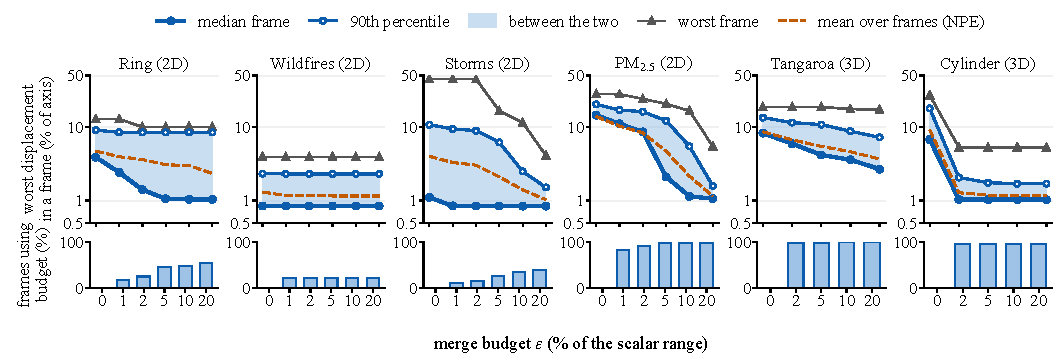
\includegraphics[width=\textwidth]{figures/budget_response_v30.pdf}
\caption{How a merge budget acts across frames. For each sequence and budget, the worst displacement of every frame is summarized over all frames: the median frame, the 90th percentile and the worst frame (log scale), and the mean over frames, which is NPE (dashed). Bottom: the share of frames whose attained merge error is positive, that is, frames that use the budget. Every frame stays within its budget. The volumes were not run at 1\%.}
\label{fig:budget-distribution}
\end{figure*}
\subsection{How a Merge Budget Acts across Frames}\label{sec:relaxation-results}
A budget limits merge error, not displacement, so its effect depends on how many frames contain a conflict it can release (Fig.~\ref{fig:budget-distribution}). Two regimes appear. On Storms the budget acts on a tail: 35\% of the frames use the allowance at $\varepsilon=10\%$, the median displacement moves only from 1.10\% to 0.84\%, but the 90th percentile falls from 10.7\% to 2.5\% and the worst frame from 44.8\% to 11.6\%. On PM$_{2.5}$ and the volumes almost every frame contains a releasable conflict and the whole distribution moves: on PM$_{2.5}$, 97\% of the frames use a 5\% budget and the median falls from 14.5\% to 2.1\%; on Cylinder, 2\% already lowers the median from 6.8\% to 1.0\%; on Tangaroa the median falls from 8.2\% to 3.6\% at 10\% and to 2.7\% at 20\%. The share of frames that use the budget is thus itself a diagnostic of how strongly a sequence entangles hierarchy and space. Exact has zero merge error on every input; Balanced attains at most 0.982, 4.421 and 9.985\% on Ring, Wildfires and Storms, and every frame passes the continuous and raster checks. Supplementary Fig.~S4 samples the budget more finely.

\begin{figure*}[!tb]
\centering
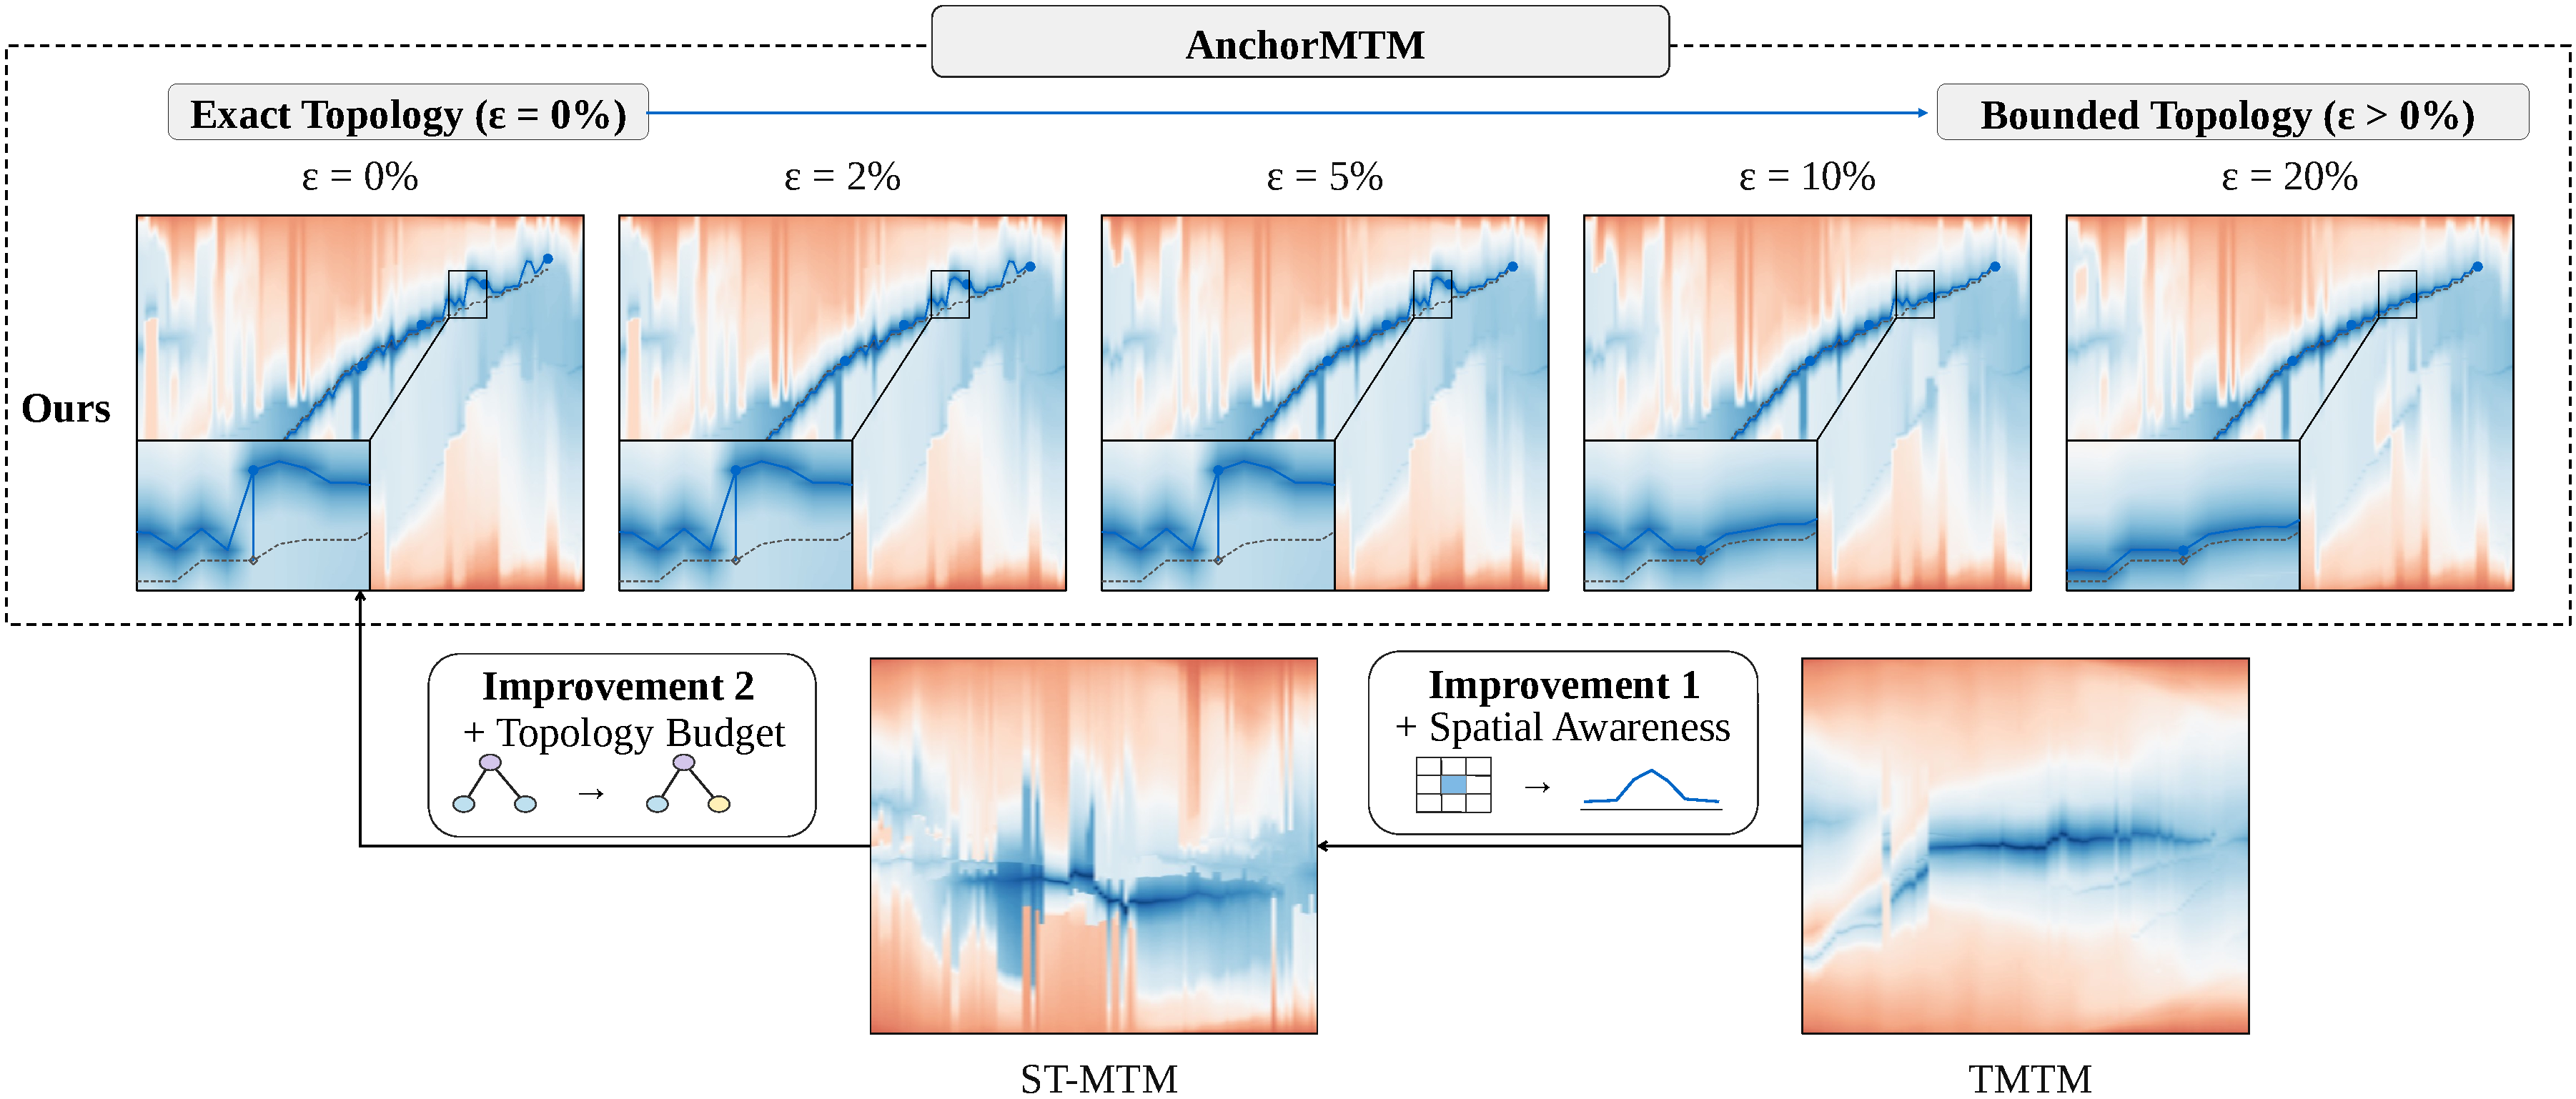
\includegraphics[width=\textwidth]{figures/anchor_storms_budget_maps.pdf}
\caption{Storms event window, frames 355--460, drawn by AnchorMTM at five budgets and by TMTM and ST-MTM on the same fields and trees, on one $[-35,35]$\,hPa scale. The lower comparison illustrates two improvements: ST-MTM adds pairwise spatial distances to TMTM's tree order, and AnchorMTM gives the axis one fixed direction and controls the merge levels it may change. The dashed curve in the insets is the reference trajectory of the tracked storm.}
\label{fig:storms-budget-profiles}
\end{figure*}
\subsection{Reading Anchored Maps}\label{sec:case-studies}
\paragraph{A storm crossing the North Atlantic.} Figures~\ref{fig:storms_overview} and~\ref{fig:storms-budget-profiles} follow one low from the open Atlantic to Scandinavia between 16 and 19 December 1999. In the AnchorMTM maps its band rises steadily along the axis, and the rise is the storm's eastward motion, while the profile still shows how it merges with the neighboring lows. TMTM aligns subtrees by temporal overlap and ST-MTM places them by relative distance, so both keep the storm near the same height and its motion cannot be read from the map. The budget changes the picture locally: at 0, 2 and 5\% the maps coincide in this window, while 10 and 20\% release the remaining conflict and move the storm onto its reference trajectory (insets).

\paragraph{Vortex shedding behind a cylinder.} The anchored default places the shed vortices at their streamwise positions (Fig.~\ref{fig:volume-gallery}). When the wake changes regime is read better if the hierarchy is given priority: an exploratory variant that freezes the leaf order of a compact TMTM layout and guides the anchors toward it separates five stages of the wake, but gives up the spatial axis (Supplementary Section~S4.8). The two readings complement each other. Supplementary Fig.~S7 reads an hourly PM$_{2.5}$ episode in the three maps.

\subsection{Implementation and Verification}
Each rendered column is checked against the fixed-label merge matrix of its source tree, together with interval order, capacity, gaps and anchor slack, and the bounds and baseline inversion errors are recomputed independently (Supplementary Section~S4.10). Ordering and placement take 0.15--3.32\,s per benchmark sequence and 200\,s for the 744-frame PM$_{2.5}$ sequence on an Apple M4 (Supplementary Table~S1).
